\documentclass[12pt,a4paper]{article}

\usepackage[utf8]{inputenc}
\usepackage[french]{babel}
\usepackage[T1]{fontenc}

\makeatletter
\title{SYSG5 : Exploitation de failles de sécurité LINUX}
\let\Title\@title
\author{Antoine Ghigny - 56359}          \let\Author\@author
\date{24/11/2022}           \let\Date\@date
\makeatother

\usepackage{titling}

\usepackage[a4paper,
            bindingoffset=0.2in,
            left=1in,
            right=1in,
            top=1in,
            bottom=1in,
            footskip=.25in]{geometry}
            
\usepackage{blindtext}
\usepackage{hyperref}
\usepackage{graphicx,color, caption}
\usepackage{epsfig}
\usepackage{fancyhdr}
\usepackage{listings}
\usepackage{color}
\usepackage{makeidx}
\usepackage{verbatim}



\graphicspath{ {./images/} }

% Valeurs par défaut le lstset
\lstset{language={},%C,Assembleur, TeX, tcl, basic, cobol, fortran, logo, make, pascal, perl, prolog, {}
	literate={â}{{\^a}}1 {ê}{{\^e}}1 {î}{{\^i}}1 {ô}{{\^o}}1 {û}{{\^u}}1
		 {ä}{{\"a}}1 {ë}{{\"e}}1 {ï}{{\"i}}1 {ö}{{\"o}}1 {ü}{{\"u}}1
		 {à}{{\`a}}1 {é}{{\'e}}1 {è}{{\`e}}1 {ù}{{\`u}}1 
		 {Â}{{\^A}}1 {Ê}{{\^E}}1 {Î}{{\^I}}1 {Ô}{{\^O}}1 {Û}{{\^U}}1
		 {Ä}{{\"A}}1 {Ë}{{\"E}}1 {Ï}{{\"I}}1 {Ö}{{\"O}}1 {Ü}{{\"U}}1
		 {À}{{\`A}}1 {É}{{\'E}}1 {È}{{\`E}}1 {Ù}{{\`U}}1,
	commentstyle=\scriptsize\ttfamily\slshape, % style des commentaires
	basicstyle=\scriptsize\ttfamily, % style par défaut
	keywordstyle=\scriptsize\rmfamily\bfseries,% style des mots-clés
	backgroundcolor=\color[rgb]{.95,.95,.95}, % couleur de fond : gris clair
	framerule=0.5pt,% Taille des bords
	frame=trbl,% Style du cadre
	frameround=tttt, % Bords arrondis 
	tabsize=3, % Taille des tabulations
%	extendedchars=\true, % Incompatible avec utf8 et literate
	inputencoding=utf8,
	showspaces=false, % Ne montre pas les espaces 
	showstringspaces=false, % Ne montre pas les espaces entre ''
	escapechar=°}  % Caractère d'échappement, permet des commandes latex dans la source


\begin{document}
\maketitle 
   \newpage
   \tableofcontents
    \newpage
   \section{Introduction (à modifier)}
   \begin{flushleft}
       \noindent Dans ce rapport, je vais détailler plusieurs failles de sécurité. L'origine de ces failles, la raison de leurs existence. Le moyen de les exploiter mais également comment s'en protéger.
       \item Je vais tout d'abord parler d'une faille permettant à n'importe quel utilisateur du système d'augmenter ses privilèges à ceux de root. Une faille présente depuis 12 ans et corrigée début 2022. Il s'agit de la faille CVE-2021-4034, plus connue sous le nom de PwnKit.
       \item Je vais ensuite expliquer comment modifier le mot de passe root depuis le grub sans le connaître via le GRUB. Pourquoi ce n'est pas sécurisé et commment s'en protéger. 
       \item Je vais dans le cadre de ce cours du système utiliser des concepts tels que l'écriture hors limite, la pile d'appels, l'insersion de données malveillantes les variables d'environement, l'utilisation et le fonctionnement du grub dans le cadre d'une attaque physique.
   \end{flushleft}

   \section{Préparation de l'environnement}
    \subsection{Installation de l'image disque}
    \begin{flushleft}
       \noindent Afin de pouvoir tester certaines failles qui ont été corrigées via des mises à jour. J'ai réalisé un l'environnement suivant. 
       \item OS : 
       \begin{itemize}
           \item  Debian 10
           \item Image: \href{https://cdimage.debian.org/mirror/cdimage/archive/10.7.0/amd64/iso-dvd/debian-10.7.0-amd64-DVD-1.iso}{debian-10.7.0-amd64-DVD-1.iso } \cite{CVE2021350:online}
           \item System info: Linux debian 4.19.0-14-amd64 \#1
       \end{itemize}
       \item SUDO : 
       \begin{itemize}
           \item Package version: 1.8.27-1+deb10u2
           \item Checksum (sha256): ca4a94e0a49f59295df5522d896022444cbbafdec4d94326c1a7f333fd030038
           \item Source code: \href{https://www.sudo.ws/dist/sudo-1.8.27.tar.gz}{sudo-1.8.27.tar.gz} \cite{CVE2021350:online}
       \end{itemize}

       \subsection{Vérification de la copie}
       \item Il est important de vérifier l’intégrité et l’authenticité de votre image ISO.
       \item Le test d’intégrité confirme que votre image ISO a été proprement téléchargée et qu’elle est une copie exacte du fichier présent sur le miroir de téléchargement. Une erreur pendant le téléchargement peut corrompre l’image et engendrer des problèmes aléatoires pendant l’installation.
       \item Pour vérifier l’intégrité de votre image ISO, générez sa somme de hachage SHA256 et comparez la à la somme qu'il devrait avoir : \textbf{ca4a94e0a49f59295df5522d896022444cbbafdec4d94326c1a7f333fd030038}
        \begin{lstlisting}
sha256sum -b debian-10.7.0-amd64-DVD-1.iso
        \end{lstlisting}
        \item Sil les sommes correspondent, votre image ISO a été proprement téléchargée. Sinon téléchargez la à nouveau. 
       
       \subsection{Création d'un stick USB}
       \item Munissez-vous d'une clé USB, branchez-là sur un ordinateur.
       \item Placez le stick USB, attendez une seconde et tapez la commande \textbf{dmesg}
       \item Les dernières lignes affichées de cette commande vous donnent le nom du pilote associé au stick (sdb,
sdc, sdd, ...), par exemple sdb.
        \item Entrez la commande suivante : 
        \begin{itemize}
            \item \textbf{Downloads/debian-10.7.0-amd64-DVD-1.iso} correspond au chemin où se situe l'image disque téléchargée plus tôt. 
            \item \textbf{/dev/sdb} correspond quant à lui au nom du pilote asocié à votre disque. : 
        \end{itemize}
        \begin{lstlisting}
sudo dd bs=4M if=Downloads/debian-10.7.0-amd64-DVD-1.iso of=/dev/sdb conv=fdatasync
        \end{lstlisting}
        

       \subsection{Configuration du réseau}
       \item Pour configurer le réseau avec celui de l'école j'ai encodé les éléments suivant
       \begin{itemize}
           \item IP : 10.0.255.20
           \item Gateway : 10.0.255.115
           \item Masque de sous réseau : 255.255.255.0
           \item DNS : 195.238.2.21 195.238.2.21 8.8.8.8
       \end{itemize}
       \subsection{Configuration des partitions}
       \item Les partitions à paramètrer ont été les suivantes : 
       \begin{itemize}
           \item 1 : Changer la partition de fat16 à EFI
           \item 2 : biosgrub
           \item 5 : swap
           \item 6 : 15 GB : / 
           \item 7 : 10 GB : /home
           \item 8 : 10GB : /usr 
       \end{itemize}
       \subsection{Configuration de l'environnement de travail}
       
       \item Et enfin j'ai ajouté l'utilisateur au groupe sudo comme c'est généralement le cas sur un environnement linux.
       \begin{lstlisting}
su -
addgroup user sudo
       \end{lstlisting}
        \subsubsection{Installation des packets requis}
       \item Afin de pouvoir installer des packets, il faudra update pour télécharger les informations des packages des sources configurées. 
       \item Pour cela, accédez en écriture au fichier \textbf{/etc/apt/sources.list} via la commande ci-dessous ou exécutez le script mit à disposition.

       \begin{lstlisting}
nano /etc/apt/sources.list
       \end{lstlisting}      

       \begin{figure}[!h]
         \centering
               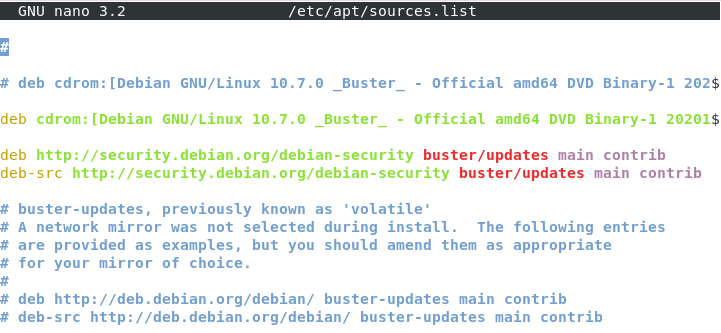
\includegraphics[scale=0.6]{sources.list}
            \caption{Le contenu du fichier contant les sources debian après l'installation}
        \end{figure}
        
       \item Mettez en commentaire la ligne concernant le cdrom installé [Debian GNU/Linux...]. Sinon il vous sera demandé d'insérer le disque qui a permis l'installation comme ci-dessous.             

        \begin{figure}[!h]
         \centering
            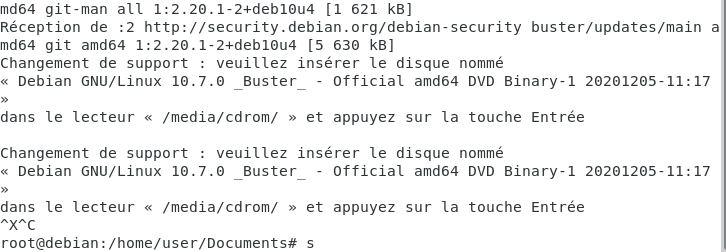
\includegraphics[scale=0.6]{cdrom}
            \caption{Erreur sans l'ajout des sources}
        \end{figure}
       \item Ajoutez au fichier les 4 lignes suivantes : 
       \begin{lstlisting}
deb http://deb.debian.org/debian/ buster-updates main contrib
deb-src htp://deb.debian.org/debian/ buster-updates main contrib
deb http://ftp.debian.org/debian/ buster main contrib
deb-src http://ftp.debian.org/debian/ buster main contrib
       \end{lstlisting}
    \item Cela permettera de télécharger depuis les sources complètes de debian. 
    \item Enfin, sauvez le fichier et \underline{téléchargez les packets} via la commande suivante
    \begin{lstlisting}
sudo apt-get update
    \end{lstlisting}
    \item Vous pouvez maintenant installer des packets tels que "git", "make" ou encore "gcc".
    \item Votre environnement de développement est maintenant prêt.
   \end{flushleft}

   \section{Privilege Escalation : Pwnkit}   		
		\subsection{Origine de la faille}   
   		\begin{flushleft}
   			\noindent Cette faille va s'intéresser à l'utilisation de la commande \textbf{pkexec} qui fait partie de la bibliothèque polkit. L'appel système pkexec est apparu en 2009 et inclus dans pratiquement toutes les distributions linux actuelles.
   			\item Cette faille de sécurité est présente depuis 12 ans et récemment mise en évidence par l'équipe de recherche Qualys en février 2022. \cite{qualys}
   			\item Cette faille permet à n’importe quel attaquant qui possède un compte sur un système linux de devenir le root du système.
            \subsection{A quoi sert la bibliothèque Polkit et en particulier l'appel système pkexec ? }
            \begin{flushleft}
                \noindent Polkit (anciennement PolicyKit) est une bibliothèque logicielle libre permettant aux applications s'exécutant avec des droits restreints d'interagir avec des services privilégiés du système. À la différence d'autres méthodes permettant une élévation des privilèges comme sudo, le processus ne se voit pas attribuer les droits superutilisateur, ce qui permet un contrôle fin au niveau du système de ce que peuvent faire ou non les utilisateurs. \cite{policyki47:online}
                \item C'est un logiciel moderne actuellement privilégié par les développeurs d'environnements graphiques grâce à la sécurité qu'il fournit, en effet il fonctionne selon le principe suivant : 
                \item Un programme (démon) s'exécute en arrière-plan (sans fenêtre), et dispose des droits root.
                \item Les applications sont invitées à lui demander les droits nécessaires pour effectuer des opérations spécifiques.
                \item PolKit saura quoi répondre en fonction des "policy" paramétrées (des configurations qui définissent qui peut faire quoi, et quel logiciel a besoin de quels privilèges).
                \item Cela évite donc de lancer des programmes en tant que super-utilisateur, ça évite également d'utiliser sudo pour des commandes n'en ayant pas besoin ou ne le supportant pas, la sécurité est donc accrue, et moins d'actions sont requises de la part de l'utilisateur (ce sont les applications qui demandent les droits, pas l'utilisateur).

                \item Polkit est intégré aux distributions Ubuntu (depuis la version 8.04), Fedora (depuis la version 8), Mandriva (depuis la version 2008.1) et OpenSUSE (depuis la version 10.3).
                \subsubsection{Utilisation des "policy"}
                \begin{flushleft}
                    \noindent Pour gérer les règles il faut donc éditer les fichiers de configuration avec les droits d'administration. La configuration se fait avec des règles et des actions :
                    \begin{enumerate}
                        \item Les Actions sont définies dans des fichiers XML .policy situés dans \textbf{/usr/share/polkit-1/actions} 
                        \item Les règles d'autorisation sont définies dans les fichiers .rules JavaScript. On les trouve à deux endroits : \cite{PartVMan11:online}
                        \begin{enumerate}
                            \item \textbf{/usr/share/polkit-1/rules.d} pour les paquets tiers peuvent utiliser (bien que peu, voire aucun, ne le fasse)
                            \item \textbf{/etc/polkit-1/rules.d} pour la configuration locale.
                        \end{enumerate}
                    \end{enumerate}
                \end{flushleft}
                \subsubsection{Utilisation classique de l'appel système pkexec (à modifier)}
                \begin{flushleft}
                    \begin{lstlisting}
 pkexec --user <username> <command>
                    \end{lstlisting}
                     \item \textbf{pkexec} Un programme de ligne de commande qui permet à un utilisateur d’exécuter des commandes comme un autre utilisateur. Si le programme est appelé sans argument utilisateur, la valeur par défaut est d’exécuter la commande en tant que root. Cette commande est très similaire à la commande sudo dans cet aspect. \cite{CVE2021425:online}
                \end{flushleft}
                \subsubsection{Quelle est la différence entre pkexec et sudo ?}
                \begin{flushleft}
                    \noindent Dans le concept, ils font la même chose, permettant à un utilisateur d'exécuter un autre programme en tant qu'autre utilisateur
                    \item Sudo et son frère aîné su, vous donnent un contrôle total sur tout.
                    \item Pkexec fait partie d'un système d'outils plus vaste appelé Polkit. Cela prend un peu de temps pour le configurer, mais une fois sur place, il donne un contrôle beaucoup plus fin.
                    \item C'est une bonne idée pour s'isoler de certains dangers et avoir l'accès complet à tout dans le système.
                \end{flushleft}
            
            \end{flushleft}
   		\end{flushleft}
   		\subsection{Comment la faille fonctionne-elle ? (à modifier) }
   		\begin{flushleft}
   			\noindent \textbf{pkexec} est une commande comme les autres, on peut lui passer des arguments
   			\item Mais il y a un gros problème dans la façon dont il va être implémentée, si l'argument argc est à la valeur NULL, le fonctionnement de pkexec va être déréglé. 
   			\item En manipulant des variables d'environnements et en créant des dossiers qui portent le même nom que ce qu'on va inscrire dans les variables d'environnement. Il est possible de charger un bout de code à un endroit contrôlé par l'attaquant. 
   		\end{flushleft}
   		
   		\subsection{Détails techniques sur la faille (à compléter) }
   		\begin{flushleft}
            \subsubsection{Ce que fait la faille}
                \begin{flushleft}
                     \noindent Pkexec de Polkit présente une vulnérabilité de corruption de mémoire conduisant à une escalade locale des privilèges
                    \item Cette vulnérabilité survient en raison d’un descripteur non sécurisé de la validation des arguments ce qui entraîne une écriture hors limite dans les paramètres envp (variables d’environnement).
                    \item Étant donné que pkexec est un binaire SUID, il s’exécute avec les privilèges root par défaut si aucun autre utilisateur ne le spécifie explicitement. 
                    \item Par conséquent, l’attaquant peut le manipuler pour exécuter du code avec des privilèges root.
                \end{flushleft}
            \subsubsection{Contexte et concepts à connaître}
            \underline{Les arguments dans la fonction main() : }
                \item On peut définir une fonction main dans les systèmes UNIX en utilisant 3 arguments.
                \begin{lstlisting}
int main(int argc, char* argv[], char *envp[])
                \end{lstlisting}
                \item \textbf{argc : } Donne le nombre d'arguments dans la ligne de commande
                \begin{enumerate}
                    \item Entier qui représente la taille du tableau d’arguments,argv, qui est passé à la fonction main(). Le tableau argv est de longueur argc et se compose d’éléments commençant par argv[0] jusqu’à argv[argc-1].
                    \item Le dernier élément est un pointeur NULL, qui garantit que la liste se termine lorsqu’elle atteint sa fin.
                \end{enumerate}
                \item \textbf{argv : } Est un tableau de pointeur de caractère représentant les arguments individuels fournis sur la ligne de commande.
                 \begin{enumerate}
                        \item Ses éléments sont les arguments de ligne de commande transmis au programme lorsqu’il a été exécuté à partir de la ligne de commande. 
                        \item Le nom de fichier du programme en cours d’exécution est également inclus dans le tableau et constitue son premier élément.
                        \item Ainsi, par exemple, si nous voulons exécuter une commande cat, avec deux arguments supplémentaires – foo et bar – nous écrirons la commande ’cat foo bar'. Dans ce cas, argc, qui est la longueur de ce tableau, est3, et argv a trois éléments, « cat », « foo » et « bar ».
                \end{enumerate}
                \item \textbf{envp : } Donne les variables d'environnement du programme. 
                \begin{enumerate}
                    \item Cet argument permet à la fonction d’accéder aux variables d’environnement du programme, telles que la variable PATH, qui spécifie un ensemble de répertoires dans lesquels un programme exécutable appelé est recherché.
                \end{enumerate}
                
                \begin{center}
                    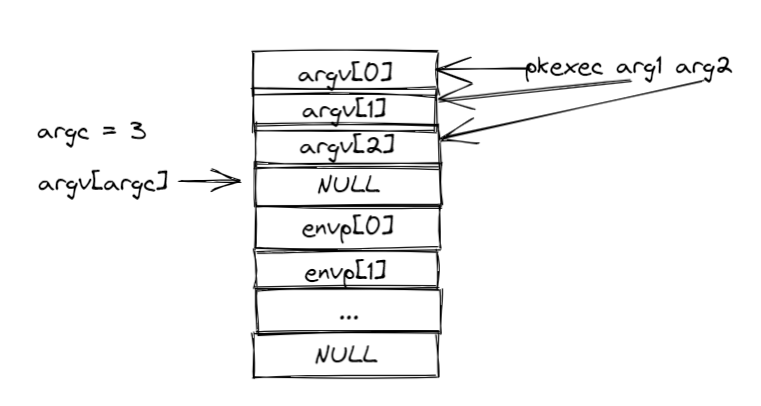
\includegraphics[scale=0.6]{main}
                \end{center}
            \underline{Ecriture hors-limite : }
                \item Les langages de programmation tels que C offrent de puissantes fonctionnalités de gestion explicite de la mémoire et d’arithmétique des pointeurs. Cependant, cela se fait au détriment de l’absence de protection intégrée contre l’accès ou l’écrasement des données dans n’importe quelle partie de la mémoire.
                \item Un exemple courant est celui des tableaux de tableaux. C’est au programmeur de vérifier s’il accède à un élément qui se trouve dans la plage d’un tableau et qui ne dépasse pas sa taille.
            \item \underline{Pile d’appels :}
                \item Il s’agit d’un concept fondamental dans le fonctionnement du logiciel. Un programme est construit à partir de plusieurs sous-routines qui s’appellent les unes les autres dans une logique particulière.
                \item Parmi les données stockées sur la pile pour la fonction main(), se trouvent les tableaux \textbf{argv} et \textbf{envp}.
                \item En fait, ils sont situés juste à côté l’un de l’autre, de sorte que la fin de argv,argv[argc], est adjacente au début de envp,envp[0].

            \item \underline{iconv\_open (à modifier) }
                \item Il s’agit d’une commande Linux qui peut être utilisée comme fonction dans le code C. 
                \item Son but est de trouver une bibliothèque appropriée qui peut convertir une chaîne donnée d’un codage à un autre (par exemple UTF-8 à UTF-16)
                \item L’un des moyens par lesquels iconv\_open() trouve une telle bibliothèque est de lire n’importe quel fichier présent dans la variable d’environnement GCONV\_PATH et de l’exécuter.
                \item Compte tenu de sa capacité à contenir des références à des bibliothèques arbitraires qui sont ensuite exécutées, la variable GCONV\_PATH était notamment connue pour faciliter les exploits d’exécution de code. 
                \item C’est pour cette raison que la variable d’environnement GCONV\_PATH est omise lors de l’exécution de programmes tels que pkexec, qui traitent de l’exécution de commandes avec des privilèges élevés temporaires.
            \subsubsection{Explication ligne par ligne, pourquoi une écriture hors limite est provoquée et d'où provient la faille dans le code source de pkexec}
                \item  Vous trouverez ci-dessous une partie de la fonction main() de pkexec sur une version vulnérable à la faille, à laquelle sont donnés les arguments ci-dessus lorsque la ligne de commande est exécutée :
                \item La fonction main{} dans pkexec a une boucle for à la ligne 534, \textbf{l'initialisation de cette boucle commence par 1} jusqu'au nombre d'arguments dans la ligne de commande (argc).
                \begin{lstlisting}
534 for (n = 1; n< (guint) argc; n++)
535 {
536   if (strcmp (argv[n), "-help") = 0)
...
548     if (n >= (guint) argc)
549     {
550       usage (argc, argv);  
551       goto out;
552     }
553
554     if (opt_user != NULL)
...
564     {
565        break;
566     }
567 }
                \end{lstlisting}
                \item Ce qui veut dire que si nous passons à execve un NULL. argc serait égal à 0. La boucle sera terminée et n serait à 1.
                \item La ligne 610 argv[n] dépasse la longueur du tableau (qui est vide), ce qui signifie que le code lit au-delà des limites du tableau comme ci-dessous.
                \begin{lstlisting}
610 path = g_strdup (argv[n]);
629 if (path [0] != "/')
630 {
...
632     s = find_prog ram_in_path (path);
...
639     argv[v] = path = s;
640  }
                \end{lstlisting}
                \item À la ligne 610, le chemin du programme à exécuter est lu hors limites à partir de argv[1] (c’est-à-dire envp[0]), et pointe vers « un fichier » comme vu ci dessous.
                \begin{center}
                    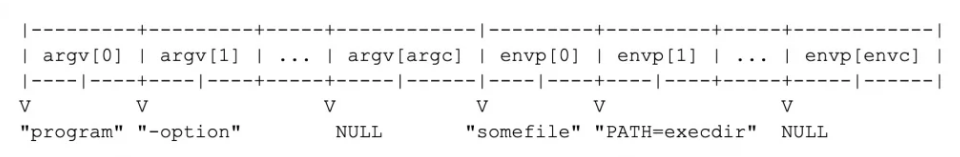
\includegraphics[scale=0.4]{image}                
                \end{center}
                \item La ligne 632 appelle la fonction g\_find\_program\_in\_path() et tente de trouver le chemin absolu du nom du programme dans le chemin, qui nous est maintenant inconnu, car il a été extrait d’une valeur lue hors limites. 
                \item Supposons qu’il existe un fichier portant le même nom que la valeur du chemin, son chemin absolu sera maintenant réécrit dans argv[n], accédant à nouveau au tableau argv au-delà de ses limites, ce qui déclenche une écriture hors limites (ligne 639).
                \item À la fin de ce flux, un emplacement mémoire en dehors du tableau argv, qui pourrait éventuellement pointer vers une chaîne qui est un nom de fichier, est remplacé par le chemin absolu du fichier.

                \item Comme décrit précédemment, la fonction main(), comme toutes les autres fonctions, peut accéder à ses arguments et variables grâce à la pile d’appels, qui les stocke de manière ordonnée. Les tableaux argv et envp sont stockés côte à côte, comme indiqué ci-dessous.
                \item  Etant donné qu'argc est égal à 0 cela signifie que argv[1] pointe vers envp[0] comme illuctré ci-dessous
                \begin{center}
                    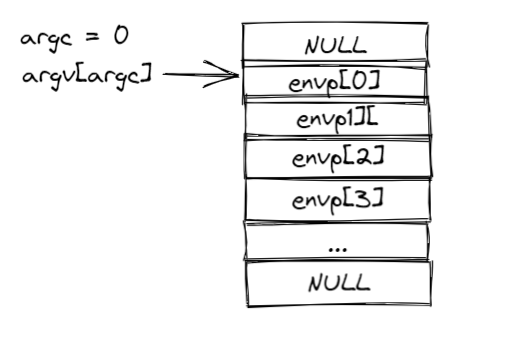
\includegraphics[scale=0.7]{ecriture environnement.png}
                \end{center}
                \item Maintenant, la question est à nouveau de savoir si nous pouvons contrôler la valeur accessible hors limites, envp[0]? 
                \item Eh bien, oui, envp[0] contient la première variable d’environnement qui est passée à pkexec lors de son exécution. 
                \item De plus, nous pouvons contrôler les variables d’environnement que nous voulons transmettre à pkexec lorsque nous l’exécutons. 
                \item \textbf{Ce qui signifie qu'envp[0] est sous notre contrôle.}
                
                \subsubsection{Ajout du code malicieux via notre environnement contrôlé}
                \item \underline{Utilisation de notre Call-Stack}
                     \item Maintenant, appelons pkexec avec les conditions suivantes:
                     \begin{enumerate}
                         \item Nous allons définir sa liste d’arguments sur un tableau vide \{NULL\}
                         \item Nous allons définir sa liste de variables d’environnement sur \{"unfichier »,"PATH=execdir »,NULL\}
                         \item Nous allons créer un fichier exécutable dans le répertoire execdir, situé dans notre répertoire de travail actuel.
                     \end{enumerate}
                 \begin{center}
                    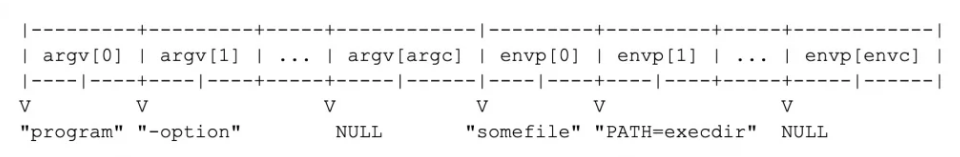
\includegraphics[scale=0.4]{image} \cite{CVE2021425:online}
                 \end{center}
                \item En d'autres termes, cette écriture hors limites nous permet de réintroduire une variable d’environnement « non sécurisée » dans l'environnement de "pkexec".
                \item Cela définit la variable d’environnement PATH, expliquée dans la section arrière-plan, pour contenir une référence au répertoire execdir. 
                \item La fonction main() va maintenant lire envp[0], qui est « unfichier », et essayer de trouver le chemin absolu de celui-ci dans le répertoire courant. 
                \item Il le trouvera, comme nous l’avons créé :  \textbf{/execdir/unfichier}. Enfin, il écrasera envp[0] avec le chemin absolu execdir/unfichier.
            \item \underline{Utilisation de GCONV\_PATH}
            \item GCONV\_PATH utilise la fonction iconv\_open pour exécuter le fichier exécutable répertorié dans la variable d’environnement GCONV\_PATH.
            \item Malheureusement pour nous, le répertoire GCONV\_PATH est omis de l’environnement de pkexec lors de son exécution, en raison de ses problèmes de sécurité connus expliqués plus tôt.
            \item Mais maintenant, ayant le contrôle sur envp[0], il est possible d'insérer GCONV\_PATH dans l'environnement de pkexec. Voici comment faire.
            \begin{enumerate}
                \item Nous allons définir sa liste d’arguments sur un tableau vide \{NULL\}
                \item Nous allons définir sa liste de variables d’environnement sur \{"exploit", " PATH=GCONV\_PATH=. ", NULL\}
                \item Nous allons créer un répertoire appelé GCONV\_PATH=.
                \item Nous allons créer un exploit de fichier exécutable, situé sous CONV\_PATH=. , de sorte que le chemin d’accès du fichier soit GCONV\_PATH=./exploit.
                \item Ce fichier contiendra un code simple qui exécute un shell sous les privilèges root.
            \end{enumerate}
            \begin{center}
                \includegraphics[scale=0.4]{pile d'exécution GCONV_PATH} \cite{CVE2021425}
            \end{center}
            \item Cela définit la variable d’environnement PATH pour qu’elle contienne une référence à au répertoire GCONV\_PATH=. 
            \item La fonction main() va maintenant lire envp[0], qui est « exploit », et essayer de trouver le chemin absolu de celui-ci dans la liste desrépertoires PATH. 
            \item Il le trouvera, car nous l’avons créé sous le répertoire GCONV\_PATH=. 
            \item Enfin, il écrasera envp[0] avec le chemin absolu de GCONV\_PATH=./exploit.
            \item Nous avons maintenant introduit la variable d’environnement GCONV\_PATH exploitable dans l’environnement de pkexec. 
            \item La dernière chose à faire est de déclencher d’une manière ou d’une autre iconv\_open et de l’utiliser le répertoire GCONV\_PATH pour charger et exécuter notre fichier malveillant.
            \item \underline{Exploitation de la fonctionnalité de validation des entrées de pkexec}
            \item Pour cela pkexec dispose de beaucoup de conditions pour valider l'entrée utilisateur.
            \item Lorsqu’il rencontre une syntaxe incorrecte ou des valeurs non valides dans les arguments de ligne de commande qui lui sont transmis, ou dans les variables d’environnement qui lui sont données, il imprime un message d’erreur indicatif à l’aide de la fonction g\_printerr() de Glib (une bibliothèque libre qui peut notamment gérer les erreurs d'appels dans notre cas).
            \item Cette fonction affiche par default les messages en codage UTF-8. Dans notre cas, la variable d'environnement CHARSET n'est pas en UTF-8. C'est maintenant que nous allons utiliser la fonction iconv\_open décrite plus tôt pour convertir la sortie UTF-8 en UTF-16.
            \item La fonction va rechercher le fichier descripteur de conversion qui sera répertorié alors dans la variable d'environnement CONV\_PATH.
            \item C'est de cette manière que nous allons forcer pkexec à exécuter notre fichier malveillant répertorié sous le répertoire GCONV\_PATH.


            \subsubsection{En résumé : }
            \item Nous allons appeler pkexec avec les conditions suivantes
            \begin{enumerate}
                \item Définir sa liste d'argument sur un tableau vide
                \item Définir sa liste de variables d'environnement sur \{"exploit", "PATH=GCONV\_PATH=.", "SHELL=/not/in/etc/shells", "CHARSET=NOT\_UTF8", NULL\}
                \item Nous allons créer un répertoire GCONV\_PATH=.
                \item Nous allons créer un exploit de fichier exécutable, situé sous le répertoire GCONV\_PATH, de sorte que le chemin d'accès de GCONV\_PATH soit GCONV\_PATH=./exploit
                \item Ce fichier contiendra un code simple qui exécute un shell sous les privilèges root.
                
            \end{enumerate}
            \begin{center}
                \begin{figure}
                    \caption{Pile d'appel de pkexec de notre programme \cite{CVE2021425:online}}
                    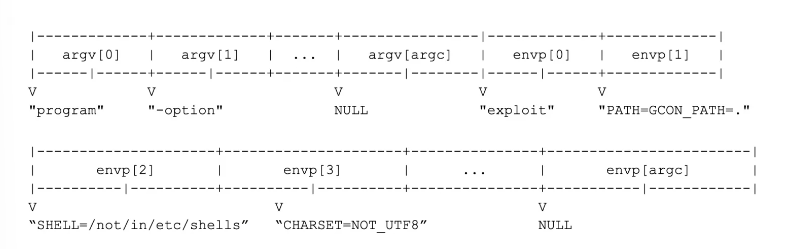
\includegraphics[scale=0.5]{pile d'appel programme final} 
                 \end{figure}
            \end{center}
            \item pkexec va accéder à envp[0] et comme vu au dessus, va aller au chemin absolu de GCONV\_PATH=./exploit, où se trouve notre fichier malveillant et le réécrire dans envp[0].
            \item Ensuite il procédera à la validation des variables d'environnement que nous avons fournies. Une par une jusqu'à arriver à celle située dans envp[2].
            \item Comme il ne remplis par les conditions d'une valeur de chemin d'accès au SHELL valide. Il va affichera une erreur à l'aide de la fonction g\_printerr(). Ce qui aura pour conséquence de vérifier la variable d'environnement CHARSET, que nous avons renseignée avec la valeur "NOT\_UTF8". Comme il ne s'agit pas d'un codage UTF-8 il appelera iconv\_open() pour l'aider à convertir l'encodage du message d'erreur à la valeur "NOT\_UTF-8".
            \item La fonction iconv\_open() fera référence au fichier de conversion située alors dans la variable d'environnement GCONV\_PATH qui contient notre fichier d'exploitation malveillant. iconv\_open charge et exécute l'exploit et nous voilà sur un shell disposant des droits administrateur.
             
   		\subsection{Comment savoir si la faille est exploitable sur le système ?}
   		La \textbf{version de pkexec} doit être inférieure à \textbf{0.105}. Il est possible de vérifier cela sur la machine de la victime en tapant la commande ci dessous : 
\begin{lstlisting}
pkexec --version
\end{lstlisting}
    \end{flushleft}
    \newpage
   		\subsection{Démonstration}
			\subsubsection{Le code C (à modifier) } 
			\lstinputlisting{../Code/PwnKit/exploit.c}  
			\subsubsection{Ce fichier contiendra un code simple qui exécute un shell sous les privilèges root} 
			\lstinputlisting{../Code/PwnKit/pwnkit.c} 
			\subsubsection{Le makefile qui s'occupe de créer les fichiers et répertoires et compile le programme}  
			\lstinputlisting{../Code/PwnKit/Makefile}
			\subsubsection{Le script qui permet d'exécuter le programme et d'effectuer une Demo de la faille} 
			\lstinputlisting{../Code/PwnKit/Demo}  

			\subsubsection{Script qui permet d'exécuter la faille}   	
			\lstinputlisting{../Code/PwnKit/Demo}
            
		\subsection{Comment a été corrigée cette faille (à modifier)}
            \begin{flushleft}
                \noindent Cette faille a été corrigée dans la version 0.105 de pkexec.
                \item Ont été ajouté à plusieurs endroits du code source de pkexec, des moyens de vérifier que le nombre d'élements entré dans la commande est supérieur à 1. Si ce n'est pas le cas, sortir du programme. 
                \item Ce qui fera sortir du programme tout utilisateur malveillant tendant d'exécuter pkexec en lui donnant NULL comme liste d'arguments et ainsi exécuter une faille de dépassement de mémoire. \cite{pkexeclo25:online} 
                \begin{center}
                    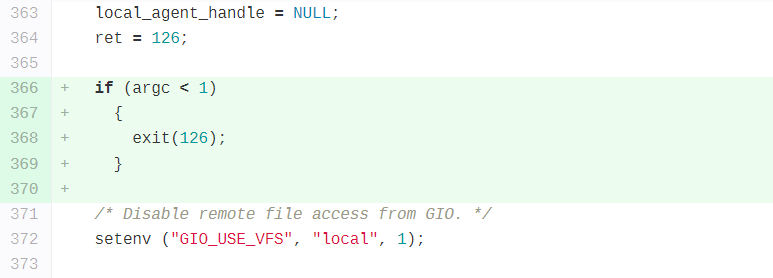
\includegraphics[scale=0.5]{verifargcsize}
                    \cite{securitytrack:online}
                \end{center}
                \item Il y a maintenant également une vérification que argv[n] doit être différent de NULL.
                \begin{center}
                    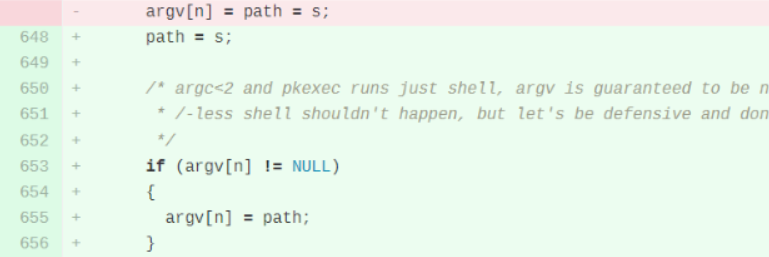
\includegraphics[scale=0.5]{verifisnull}
                    \cite{securitytrack:online}
                \end{center}
            \end{flushleft}
            
            \subsection{Comment corriger cette faille si il n'est pas possible d'ugrade la version de pkexec ? (à modifier)}
            \begin{flushleft}
                \noindent Si aucun correctif n’est disponible pour votre système d’exploitation, vous pouvez supprimer le bit SUID de pkexec à titre d’atténuation temporaire.
                \begin{lstlisting}
chmod 0755 /usr/bin/pkexec
                \end{lstlisting}
            \end{flushleft}
            \subsection{Est-il possible de vérifier les preuves d’exploitation?}
            \begin{flushleft}
                \noindent Oui, cette technique d’exploitation laisse par default des traces dans les logs (soit « La valeur de la variable SHELL n’a pas trouvé le fichier /etc/shells » soit « La valeur de la variable d’environnement [...] contient du contenu suspect »). 
                \item Cependant, veuillez noter que cette vulnérabilité est également exploitable sans laisser de traces dans les logs étant donné que l'attaquant dispose alors des permissions root sur le système.
            \end{flushleft}
    \newpage
   \section{Modifier le mot de passe administrateur sans le connaître}
        \subsection{Démonstration : GRUB}
        \begin{enumerate}
        	\item \textbf{Eteindre le pc} et après avoir rallumé l'ordinateur, ouvrir les options avancées et \textbf{ouvrir Grub}. Il s'agit d'un programme d'ammorçage du chargement d'un système d'exploitation. C'est ce qui fait le lien entre le bios et le système d'exploitation. Avant que le système ne soit chargé ou lancé.
        	\item Entrer en mode édition via la touche 'E'. Dans le menu GRUB, recherchez la ligne du noyau commençant par linux /boot/ et ajoutez cette ligne à la fin.
        	\begin{lstlisting}
rw init = /bin/bash
        	\end{lstlisting}
        	\item Sauvegardez les changements via en appuyant sur \textbf{CTRL + X} et rebooter en mode single-user mode.
        	\item Une fois cela fait, vous pouvez modifier le password administrateur via cette la commande ci-dessous, vous n'aurez qu'à entrer le nouveau mot de passe et une autre fois pour confirmer. Il suffit de redémarrer le système et le password administrateur aura été modifié. \cite{grubchangepassword:online}
        	\begin{lstlisting}
passwd root
        	\end{lstlisting}
        \item Il y a une alternative qui est CHROOT mais qui est très similaire dans son fonctionnement, c'est également en lien avec GRUB, je ne la détaillerait pas donc pas ici.
        \end{enumerate}
   \subsection{Pourquoi ça fonctionne ainsi ? Pourquoi est-il si simple de changer le mot de passe administrateur ?} 
   \begin{flushleft}
       \noindent Les mots de passe sont destinés à empêcher l'accès de l'extérieur (réseau, Internet), et ils le font. Cependant, l'accès physique est un accès root.
       \item À moins que vous ne cryptiez l'intégralité de votre partition, il est toujours possible de démarrer à partir d'un disque optique ou d'un lecteur flash et d'accéder à tous vos fichiers. De cette façon, vous pouvez également modifier les fichiers qui stockent les mots de passe des utilisateurs.
       \item Donc si quelqu'un peut toucher à votre machine, il peut y entrer.
   \end{flushleft}

   \subsection{Comment protéger le grub pour ne plus que cette faille soit possible} 
        \subsubsection{Ajouter un mot de passe à GRUB} 
        \begin{flushleft}
            \noindent Il est possible d'ajouter un mot de passe à grub.
            \item Un mot de passe sera alors requis pour modifier les entrées du menu mais pas pour démarrer les entrées de menu existantes. 
            \item Pour cela, créez un mot de passe avec la commande suivante. Vous aurez à entrer un mot de passe, confirmer et ne surtout pas oublier le mot de passe que vous avez encodé.
       \begin{lstlisting}
grub2-setpassword
       \end{lstlisting}
            \item Cette commande créera ou mettra à jour le contenu de \textbf{/boot/grub2/user.cfg} avec le mot de passe hashé. \cite{Howtopro9:online}
        \end{flushleft}
        \subsubsection{Désactiver le mode de récupération de votre choix}
        \begin{enumerate}
            \item Ouvrir dans un éditeur de texte le fichier de paramétrage du GRUB (avec des privilèges root)
        \begin{lstlisting}
sudo nano /etc/default/grub
       \end{lstlisting}
            \item Décommentez/ajoutez la ligne suivante :
            \begin{lstlisting}
GRUB_DISABLE_RECOVERY="true"
            \end{lstlisting}
            \item Enregistrez les modifications et exécutez la commande suivante :
            \begin{lstlisting}
sudo update-grub
            \end{lstlisting}
        \end{enumerate}
        \subsubsection{Protéger le bootloader GRUB}
        \begin{enumerate}
            \item Ouvrez un shell en mode root et tapez "grub"
            \item Entrez la commande "md5crypt" 
        \end{enumerate}
        \newpage
        \section{Conclusion}
        \begin{flushleft}
            \item En conclusion une faille qui tente d'exploiter des vulnérabilités de dépassement de mémoire d'applications sont des attaques très efficaces.
            \item Ces attaques concistent à exécuter du code arbitraire afin de compromètre la cible. 
            \item Dans le cas de la faille de sécurité que j'ai expliquée, son but consistait d'injecter du code malveillant dans les variables d'environnement du code permettant d'exécuter un shell avec les privilèges root.
            \item Afin de protéger le système, il est nécéssaire d'appliquer rapidement les patchs fournis par les développeurs en mettant régulièrement à jour son système. 
            \item De tenter au maximum de fiabiliser l'OS pour qu'il ne soit pas vulnérable aux dépassements de tampon. Auditer des programmes compilés à l'aide d'outils tels que BFBTester. Je ne détaillerais pas plus que ça ce programme mais il est utile pour tester de manière proactive des programmes et vérifier que ceux-ci ne provoquent pas de dépassements de mémoire.
            \item Il faut également faire attention à protéger sa machine contre les attaques physiques. Si rien n'a été fait pour sécuriser son GRUB et que l'intégralité du disque n'a pas été cypté. Un attaquant peut de manière simple obtenir l'accès root et faire n'importe quoi sur la machine.
        \end{flushleft}
        \newpage
        \nocite{*}
	\bibliography{bibliozq}
	\bibliographystyle{plain}
\end{document}
